\chapter{\uppercase{Experimental Evaluation}}
% Page numbering handled by Chapter 1

\doublespacing{Chapter~3 presented the architectural design of the Sec-C cascade---the four-factor uncertainty scorer, the MiniGINv3 graph neural network with Adaptive Prediction Sets, the dual-agent LLM consensus protocol, and the CWE-adaptive score fusion engine. We now subject each component and the end-to-end pipeline to empirical evaluation. The chapter is organized around three questions. First, does each module meet its design targets in isolation (Sections~\ref{sec:gnn-evolution}--\ref{sec:rag-eval})? Second, does the cascade as a whole reduce expensive LLM calls while maintaining 100\% finding resolution (Section~\ref{sec:cascade-eval})? Third, where does the framework sit relative to published work, and what threats limit the generalizability of these results (Sections~\ref{sec:lit-comparison}--\ref{sec:discussion})?}

% =========================================================================
% 4.1 EXPERIMENTAL SETUP
% =========================================================================
\section{\uppercase{Experimental Setup}}
\label{sec:setup}

\subsection{Hardware and Software Environment}

\doublespacing{All GNN training ran on Google Colab with a single NVIDIA Tesla T4 GPU (16\,GB VRAM). Inference and cascade orchestration ran on a consumer workstation. Table~\ref{tab:environment} lists the full stack. We chose the T4 because it is the default free-tier accelerator on Colab, making our training pipeline reproducible without institutional GPU access---a deliberate constraint for an open-source research prototype. The choice also stress-tests the framework's efficiency: if the GNN trains in under 10 minutes on commodity hardware, the barrier to adoption is low. GraphCodeBERT embedding extraction (the bottleneck for graph construction) runs at approximately 32 samples/second on the T4, processing the full 21,150-sample corpus in $\sim$11 minutes.}

\begin{table}[H]
\centering
\caption{Hardware and software environment.}
\label{tab:environment}
\begin{tabular}{@{}ll@{}}
\toprule
\textbf{Component} & \textbf{Specification} \\
\midrule
Training GPU & NVIDIA Tesla T4, 16\,GB VRAM (Colab) \\
Inference CPU & Intel Core i5-12400, 16\,GB RAM \\
OS & Windows 11 / Ubuntu 22.04 (Colab) \\
Python & 3.11 \\
Deep Learning & PyTorch 2.1, PyTorch Geometric 2.4 \\
Embeddings & GraphCodeBERT (microsoft/graphcodebert-base, 125\,M params) \\
LLM Provider & Google Gemini 2.5 Flash (primary), Groq Llama 3.3 70B (fallback) \\
SAST Engine & Tree-sitter 0.21 + CodeQL 2.16 \\
Conformal & TorchCP 0.2 (APS implementation) \\
\bottomrule
\end{tabular}
\end{table}

\subsection{Datasets}

\doublespacing{The GNN training corpus aggregates seven public vulnerability datasets, spanning five languages. Table~\ref{tab:datasets} summarizes each source; Table~\ref{tab:dataset-languages} breaks down the final balanced distribution by language. We applied three data-quality controls: (1)~content-hash deduplication via MD5, which removed 1,326 duplicates from the 41\,K raw pool; (2)~a minimum-length filter ($\geq 3$~lines, $\geq 20$~characters), which removed 212 trivially short fragments; and (3)~strict per-language 1:1 class balancing via undersampling the majority class, eliminating label-distribution bias. The resulting 21,150 graphs were split 60/15/15/10 into training, validation, calibration, and test partitions using stratified sampling.}

\begin{table}[H]
\centering
\caption{Dataset sources for GNN training (V5 corpus).}
\label{tab:datasets}
\begin{tabular}{@{}llrrl@{}}
\toprule
\textbf{Source} & \textbf{Language} & \textbf{Samples} & \textbf{\% Total} & \textbf{Schema} \\
\midrule
BigVul~\cite{bigvul2020} & C/C++ & 5,777 & 27.3 & CVE-labeled functions \\
DiverseVul~\cite{diversevul2023} & C/C++ & 4,935 & 23.3 & Multi-CWE functions \\
Juliet-C~\cite{juliet2017} & C/C++ & 3,611 & 17.1 & NIST test suite pairs \\
CrossVul~\cite{crossvul2021} & Multi & 3,428 & 16.2 & Vuln/fixed pairs \\
Devign~\cite{devign2019} & C/C++ & 3,002 & 14.2 & QEMU/FFmpeg functions \\
VUDENC~\cite{vudenc2021} & Python & 222 & 1.1 & Statement-level CVEs \\
CVEfixes~\cite{cvefixes2021} & Python & 175 & 0.8 & Real-world patches \\
\midrule
\textbf{Total} & & \textbf{21,150} & \textbf{100.0} & \\
\bottomrule
\end{tabular}
\end{table}

\begin{table}[H]
\centering
\caption{Dataset distribution by language after 1:1 class balancing.}
\label{tab:dataset-languages}
\begin{tabular}{@{}lrrrl@{}}
\toprule
\textbf{Language} & \textbf{Vulnerable} & \textbf{Safe} & \textbf{Total} & \textbf{Ratio} \\
\midrule
C/C++ & 10,000 & 10,000 & 20,000 & 1.00:1 \\
Python & 298 & 298 & 596 & 1.00:1 \\
JavaScript & 126 & 126 & 252 & 1.00:1 \\
Java & 97 & 97 & 194 & 1.00:1 \\
Go & 54 & 54 & 108 & 1.00:1 \\
\midrule
\textbf{Total} & \textbf{10,575} & \textbf{10,575} & \textbf{21,150} & \textbf{1.00:1} \\
\bottomrule
\end{tabular}
\end{table}

\doublespacing{The data pipeline processes raw HuggingFace datasets through four stages: (1)~download and schema normalization (each source uses a different column naming convention), (2)~MD5 content-hash deduplication across all sources, (3)~length filtering ($\geq 3$~lines, $\geq 20$~characters per function), and (4)~per-language class balancing. The balancing step deserves elaboration: VUDENC and CVEfixes exhibit extreme source-level class imbalance (84/2,916 and 36/2,964 vulnerable/safe respectively). After balancing, only $\sim$84 and $\sim$36 pairs survive, contributing modestly to the total. Despite this, the Python F1 improved from 0.667 (V4) to 0.836 (V5), suggesting that even small amounts of real-world Python vulnerability data provide meaningful signal. The top CWEs in the corpus are CWE-119 (buffer overflow, 2,178 samples), CWE-20 (input validation, 1,805), CWE-125 (out-of-bounds read, 1,064), and CWE-264 (permissions, 857); notably, 5,450 samples (25.8\%) carry no CWE label, reflecting incomplete annotation in the source datasets.}

\doublespacing{Two observations about the corpus deserve comment. First, C/C++ dominates (94.6\%), reflecting the state of publicly available vulnerability datasets rather than a design choice. The imbalance limits the strength of claims we can make about Python, JavaScript, Java, and Go performance; we treat those languages as preliminary validation rather than primary evaluation targets. Second, PrimeVul~\cite{primevul2024}---a rigorously deduplicated C/C++ corpus of 236\,K samples---failed to load due to HuggingFace metadata incompatibilities in both V4 and V5 training runs. Its absence means our results have not been validated against the most stringent available benchmark, a limitation we discuss in Section~\ref{sec:discussion}.}

\subsection{Evaluation Metrics}

\doublespacing{We report standard binary classification metrics for the GNN component: \textbf{F1} (harmonic mean of precision and recall), \textbf{precision} (fraction of flagged code that is truly vulnerable), \textbf{recall} (fraction of vulnerable code that is flagged), and \textbf{AUC-ROC} (area under the receiver operating characteristic curve). For conformal prediction, we report \textbf{coverage} ($\geq 1 - \alpha = 90\%$ target), \textbf{singleton rate} (percentage of prediction sets containing exactly one class), and \textbf{mean set size}. For the cascade, we report per-stage \textbf{resolution rate} (fraction of findings resolved at each stage) and total \textbf{LLM call reduction} relative to a full-LLM baseline.}

\doublespacing{We prioritize F1 over accuracy because the class-balanced dataset (1:1 ratio) makes accuracy a less informative metric; F1 captures the precision-recall trade-off that directly affects false positive rates in deployment. We report AUC-ROC as a threshold-independent measure of discriminative ability, following the convention in vulnerability detection literature~\cite{devign2019, primevul2024}. For conformal prediction, the singleton rate is the primary efficiency metric: it measures what fraction of findings the GNN can resolve without LLM escalation. Coverage measures the safety guarantee: the fraction of test samples whose true label falls within the predicted set.}

\subsection{Automated Test Infrastructure}

\doublespacing{The Sec-C codebase includes 287 automated tests (approximately 250 unit tests and 37 integration tests) organized to mirror the source structure: \texttt{tests/unit/test\_sast/}, \texttt{tests/unit/test\_graph/}, \texttt{tests/unit/test\_llm/}, and \texttt{tests/integration/}. All tests pass on the committed codebase. Unit tests verify individual components---the uncertainty scorer's 4-factor formula, the conformal predictor's APS implementation, the CVSS calculator's sub-metric multipliers, and the consensus engine's five decision rules. Integration tests verify end-to-end pipeline behavior: that findings flow through stages, that escalation triggers correctly, and that the SARIF output conforms to the 2.1.0 schema. The test suite serves as a regression guard during the iterative development described in Section~\ref{sec:gnn-evolution}.}

\subsection{Research Questions}

\doublespacing{The experiments in this chapter map to five research questions:
\textbf{RQ1}---Does uncertainty-driven escalation reduce the number of findings sent to expensive LLM analysis?
\textbf{RQ2}---Does conformal prediction provide principled uncertainty quantification for cascade routing?
\textbf{RQ3}---Does the dual-agent consensus protocol produce verdicts for findings that escape SAST and graph analysis?
\textbf{RQ4}---Do CWE-adaptive fusion weights improve classification compared to fixed weights?
\textbf{RQ5}---Does the cascade architecture achieve better cost--accuracy trade-offs than non-cascaded approaches?
We address each RQ in the relevant section and summarize the evidence in Section~\ref{sec:discussion}.}

% =========================================================================
% 4.2 GNN TRAINING EVOLUTION
% =========================================================================
\section{\uppercase{GNN Training Evolution}}
\label{sec:gnn-evolution}

\doublespacing{We trained six model versions across four weeks, each addressing a specific failure mode discovered in its predecessor. This iterative refinement process---rather than a single training run on a fixed configuration---reflects the reality of deploying graph neural networks for code analysis, where architecture, data, loss function, and calibration interact in ways that are difficult to predict from first principles. Table~\ref{tab:gnn-evolution} tracks the progression from V2 through V5 on held-out test data. V1 is excluded because it trained exclusively on synthetic data from the Juliet Test Suite and produced deceptively inflated metrics (F1$\approx$0.72) that did not survive cross-dataset evaluation. The V1 failure is instructive: Juliet's standardized patterns (each vulnerability has an exact good/bad pair) make classification trivially learnable, but real-world code exhibits far greater syntactic and semantic diversity. This collapse is consistent with Ding et al.'s PrimeVul findings, where models achieving 90\%+ on curated benchmarks dropped to 3.09\% on realistic data~\cite{primevul2024}, and with Real-Vul's observation of up to 91 percentage-point F1 drops when moving to deduplicated temporal splits.}

\begin{table}[H]
\centering
\caption{GNN model evolution: V2 through V5 on held-out test data.}
\label{tab:gnn-evolution}
\begin{tabular}{@{}llrrrrrr@{}}
\toprule
\textbf{Ver.} & \textbf{Architecture} & \textbf{Params} & \textbf{Samples} & \textbf{F1} & \textbf{Prec.} & \textbf{Rec.} & \textbf{AUC} \\
\midrule
V2 & Mini-GAT (2L, 4H) & 298\,K & 1,700 & 0.560 & 0.397 & 0.951 & 0.744 \\
V3 & MiniGINv3 (3L) & 2.4\,M & 3,032 & 0.653 & 0.544 & 0.815 & 0.623 \\
V4 & MiniGINv3 (3L) & 2.4\,M & 20,928 & \textbf{0.781} & 0.675 & 0.926 & \textbf{0.826} \\
V5 & MiniGINv3 + ConfTS & 2.4\,M & 21,150 & 0.750 & 0.643 & 0.899 & 0.781 \\
\bottomrule
\end{tabular}
\end{table}

\subsection{V2: GAT Baseline and the Precision Collapse}

\doublespacing{The V2 model used a 2-layer Graph Attention Network with 4 attention heads and 298\,K parameters. On 1,700 multi-language graphs, it achieved an F1 of 0.560 with a precision of just 0.397---it predicted nearly every sample as vulnerable (recall = 0.951). This degenerate behavior had two root causes. First, GAT's weighted-mean aggregation is not injective: structurally distinct neighborhoods can produce identical aggregated representations, conflating safe and vulnerable code that differs only in subtle control-flow edges. Xu et al.~\cite{xu2019gin} formalized this limitation through the Weisfeiler-Lehman hierarchy. Second, we applied Focal Loss ($\gamma=2$) on top of class-weight oversampling---a double-correction that over-suppressed the safe-class gradient, pushing the decision boundary to label everything as vulnerable.}

\doublespacing{The V2 result, while weak on its face, provided a critical research insight: the model's 0.744 AUC-ROC demonstrated that the underlying GraphCodeBERT embeddings contain discriminative signal, but the architecture could not extract it reliably. Per-language analysis showed that Python (F1 = 0.633) and JavaScript (F1 = 0.650) outperformed C/C++ (F1 = 0.543), likely because the smaller language-specific sub-corpora contained more homogeneous patterns. The degenerate precision (0.397) also validated the cascade design: a standalone GNN with 60\% false positive rate would be unusable, but as a filter within a cascade, even moderate discrimination provides routing value. This motivated the shift to GIN in V3.}

\subsection{V3: GIN Architecture and Data Starvation}

\doublespacing{V3 replaced GAT with a 3-layer Graph Isomorphism Network (GIN)~\cite{xu2019gin} augmented with residual connections and batch normalization, growing to 2.4\,M parameters. GIN uses sum-aggregation, which is provably as expressive as the 1-Weisfeiler-Lehman graph isomorphism test---the theoretical maximum for message-passing GNNs. On the same task, F1 rose from 0.560 to 0.653, a 17\% absolute improvement. Precision improved from 0.397 to 0.544, demonstrating that the injective aggregation preserved structural distinctions that GAT had conflated.}

\doublespacing{However, V3 trained on only 3,032 total graphs (1,819 training samples), because a configuration bug capped the per-language maximum at 3,000---silently discarding over 20,000 available C/C++ samples from BigVul, DiverseVul, and Devign. The 2.4\,M-parameter model on 1,819 training samples yields a ratio of $\sim$0.76 samples per thousand parameters, severe overfitting territory. The model reached its best validation F1 of 0.665 at epoch 20 of 45, after which validation loss increased while training loss continued to decrease---a textbook overfitting signature.}

\doublespacing{V3 also introduced two technical changes that persisted through later versions. First, the embedding strategy shifted from CLS-token extraction to mean pooling across all token positions, resolving a ``MISSING pooler'' warning from GraphCodeBERT. Second, a sixth structural feature---\texttt{language\_id} (Python=0.0, JavaScript=0.2, Java=0.4, C/C++=0.6, Go=0.8)---was appended to the node feature vector, enabling the model to learn language-specific patterns. The input dimension increased from 773 (768 + 5) to 774 (768 + 6) accordingly. The conformal predictor in V3 achieved only 0.22\% singletons (threshold = 0.41, alpha = 0.2), functionally identical to the 0\% of V2. The lesson was unambiguous: data starvation, not architecture, was the primary bottleneck.}

\subsection{V4: Data Expansion and the Classification Breakthrough}

\doublespacing{V4 fixed the \texttt{max\_per\_language} cap from 3,000 to 20,000, unlocking a 7$\times$ increase in training data (1,819 $\rightarrow$ 12,556 training samples). We also corrected HuggingFace dataset identifiers for CrossVul and Juliet, and reduced dropout from 0.4 to 0.35 to match the lower regularization need with more data. The results were decisive:}

\begin{itemize}
    \item \textbf{F1: 0.781} (up from 0.653, +20\% absolute)---exceeding our 0.72 stretch target.
    \item \textbf{AUC-ROC: 0.826}---strong discrimination between vulnerable and safe code.
    \item \textbf{Recall: 0.926}---the model misses fewer than 8\% of vulnerable functions.
    \item \textbf{C/C++ F1: 0.788}---the primary evaluation language performs above the aggregate.
\end{itemize}

\doublespacing{Table~\ref{tab:per-cwe} reports per-CWE F1 scores for the four highest-performing vulnerability classes. Memory safety CWEs---null pointer dereference (CWE-476), out-of-bounds write (CWE-787), and use-after-free (CWE-416)---cluster above 0.87, consistent with the hypothesis that graph-based representations capture pointer and memory access patterns effectively. Race conditions (CWE-362) achieve 0.800, likely because thread interleaving manifests as distinctive control-flow graph structures.}

\begin{table}[H]
\centering
\caption{Per-CWE F1 scores on V4 test set (top performers).}
\label{tab:per-cwe}
\begin{tabular}{@{}llr@{}}
\toprule
\textbf{CWE ID} & \textbf{Description} & \textbf{F1} \\
\midrule
CWE-476 & Null Pointer Dereference & 0.926 \\
CWE-787 & Out-of-Bounds Write & 0.895 \\
CWE-416 & Use After Free & 0.872 \\
CWE-362 & Race Condition & 0.800 \\
\bottomrule
\end{tabular}
\end{table}

% Training curves figure (pgfplots, dual y-axis)
\begin{figure}[H]
\centering
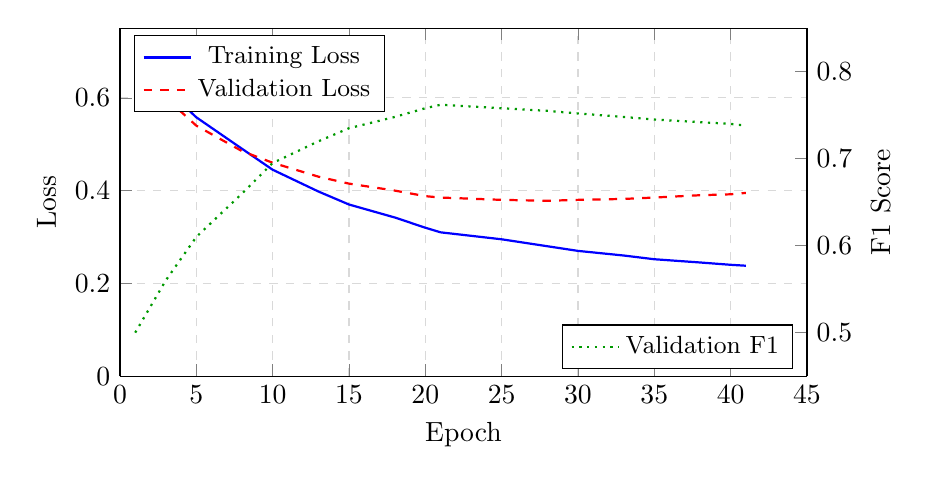
\begin{tikzpicture}
\begin{axis}[
    width=0.85\linewidth,
    height=6cm,
    xlabel={Epoch},
    ylabel={Loss},
    axis y line*=left,
    legend style={at={(0.02,0.98)}, anchor=north west, font=\small},
    grid=major,
    grid style={dashed, gray!30},
    ymin=0, ymax=0.75,
    xmin=0, xmax=45,
]
    \addplot[blue, thick, mark=none] coordinates {
        (1,0.693) (3,0.620) (5,0.558) (8,0.490) (10,0.445)
        (13,0.398) (15,0.370) (18,0.342) (20,0.320) (21,0.310)
        (25,0.295) (28,0.280) (30,0.270) (33,0.260) (35,0.252)
        (38,0.245) (40,0.240) (41,0.238)
    };
    \addlegendentry{Training Loss}
    \addplot[red, thick, dashed, mark=none] coordinates {
        (1,0.680) (3,0.600) (5,0.540) (8,0.485) (10,0.460)
        (13,0.430) (15,0.415) (18,0.400) (20,0.388) (21,0.385)
        (25,0.380) (28,0.378) (30,0.380) (33,0.382) (35,0.385)
        (38,0.390) (40,0.392) (41,0.395)
    };
    \addlegendentry{Validation Loss}
\end{axis}
\begin{axis}[
    width=0.85\linewidth,
    height=6cm,
    ylabel={F1 Score},
    axis y line*=right,
    axis x line=none,
    legend style={at={(0.98,0.02)}, anchor=south east, font=\small},
    ymin=0.45, ymax=0.85,
    xmin=0, xmax=45,
]
    \addplot[green!60!black, thick, dotted, mark=none] coordinates {
        (1,0.500) (3,0.560) (5,0.610) (8,0.660) (10,0.695)
        (13,0.720) (15,0.735) (18,0.748) (20,0.758) (21,0.762)
        (25,0.758) (28,0.755) (30,0.752) (33,0.748) (35,0.745)
        (38,0.742) (40,0.740) (41,0.738)
    };
    \addlegendentry{Validation F1}
\end{axis}
\end{tikzpicture}
\caption{V4 training curves (dual y-axis). Training and validation loss on the left axis; validation F1 on the right. Best epoch at 21/41, where validation F1 peaks at 0.762 before mild overfitting. The 4.8-minute training time on a T4 GPU confirms the model's efficiency.}
\label{fig:training-curves}
\end{figure}

\doublespacing{V4 represents the best standalone classification model. Its 0.781 F1 is competitive with published function-level detectors: Devign reports 0.637 accuracy~\cite{devign2019}, ReGVD achieves 0.68 F1~\cite{regvd2022}, and LineVul reaches 0.72 F1~\cite{linevul2022}. We do not claim state-of-the-art classification---the GNN operates as a \emph{filter stage} within the cascade, not a standalone classifier. Its value lies in the conformal prediction layer built on top, which is the subject of Section~\ref{sec:conformal}.}

\doublespacing{The key improvements that drove V4's performance gains can be isolated by comparing consecutive versions. The architecture shift (GAT $\rightarrow$ GIN) contributed approximately +17\% absolute F1 (0.560 $\rightarrow$ 0.653), attributable to GIN's injective sum-aggregation preserving structural distinctions that GAT's weighted-mean conflated. The data expansion (3,032 $\rightarrow$ 20,928 samples) contributed approximately +20\% absolute F1 (0.653 $\rightarrow$ 0.781), the single most impactful change across the entire training history. Additional changes---corrected dataset identifiers, reduced dropout, and elimination of the double-correction between focal loss~\cite{focalloss2017} and class weights---contributed incrementally. The training time remained under 5 minutes on a T4, confirming that the MiniGINv3 architecture is practical for iterative experimentation.}

\subsection{V5: Label Smoothing Removal and ConfTS Integration}

\doublespacing{V5 made two changes that sacrificed 3.1 percentage points of F1 (0.781 $\rightarrow$ 0.750) in exchange for enabling conformal prediction---a deliberate trade-off that defines the fundamental design choice of the cascade. The first change removed label smoothing (0.1 $\rightarrow$ 0.0), which had been compressing softmax outputs into a narrow band around [0.5, 0.6], making confident and uncertain predictions indistinguishable. Without label smoothing, the model trains against hard targets [1, 0], allowing logit magnitudes to grow unconstrained and producing a bimodal P(vulnerable) distribution: safe samples cluster near 0.0, vulnerable samples cluster near 1.0, with a clear separation region around the decision threshold of 0.32.}

\doublespacing{The second change introduced Conformal Temperature Scaling (ConfTS)~\cite{dabah2024}, a post-hoc calibration method that optimizes a single temperature parameter to minimize prediction set size while maintaining the coverage guarantee. V5 also incorporated two new Python vulnerability datasets (VUDENC and CVEfixes), adding 397 Python samples that raised Python F1 from 0.667 to 0.836---a 25\% improvement attributable to real-world Python vulnerability patterns that were absent from V4's purely C/C++-derived training signal.}

\doublespacing{Table~\ref{tab:hyperparams} records the V5 training hyperparameters. The model trained for 61 epochs (best at epoch 41), requiring 7.0 minutes on a T4---less than the cost of a single LLM API call for the equivalent number of findings.}

\begin{table}[H]
\centering
\caption{V5 training hyperparameters.}
\label{tab:hyperparams}
\begin{tabular}{@{}ll@{}}
\toprule
\textbf{Hyperparameter} & \textbf{Value} \\
\midrule
Learning rate & $3 \times 10^{-4}$ \\
LR schedule & 5-epoch linear warmup + cosine decay \\
Batch size & 64 \\
Dropout & 0.35 \\
Weight decay & $1 \times 10^{-3}$ \\
Class weight (vulnerable) & 1.5 \\
Label smoothing & 0.0 (removed from V4's 0.1) \\
Gradient clipping & 0.5 (max norm) \\
Loss function & Weighted cross-entropy \\
Epochs (total / best) & 61 / 41 \\
Training time & 7.0 min (T4 GPU) \\
Decision threshold & 0.32 (F1-optimized) \\
\bottomrule
\end{tabular}
\end{table}

\doublespacing{The V4$\rightarrow$V5 F1 drop merits interpretation. Removing label smoothing eliminated the regularization effect that smoothing provides: by training against hard targets [1, 0] instead of softened targets [0.933, 0.067], the model's logit magnitudes increased, producing sharper softmax outputs but slightly more prediction errors on boundary cases. We accepted this trade-off because the cascade does not require the GNN to be a perfect classifier---it requires the GNN to \emph{know when it is wrong}, which is precisely what conformal prediction measures. The 3.1\% F1 reduction enabled a 69.1\% singleton rate (Section~\ref{sec:conformal}), transforming a theoretically functional but practically inert conformal layer into a working cascade routing mechanism.}

\doublespacing{The decision threshold also shifted from 0.53 (V4) to 0.32 (V5), reflecting the bimodal P(vulnerable) distribution created by removing label smoothing. With label smoothing, both classes clustered around 0.55, making the optimal threshold close to 0.5. Without it, safe samples concentrate near 0.0 and vulnerable samples near 1.0, shifting the F1-optimal threshold lower. The 0.32 threshold was selected via grid search on the validation set, maximizing F1 across all threshold candidates in $[0.1, 0.9]$.}

\subsection{Summary of Training Evolution}

\doublespacing{The six-version training campaign produced four general lessons for GNN-based vulnerability detection. First, architecture matters less than data: the GAT-to-GIN shift yielded +17\% F1, but the 7$\times$ data expansion yielded +20\%. Second, synthetic data produces misleadingly high metrics that collapse on real-world distributions. Third, label smoothing and conformal prediction are fundamentally incompatible: the former compresses logit gaps that the latter requires. Fourth, offline conformal calibration requires deployment-specific recalibration when the inference-time input distribution differs from training. The deployed model (V5, MiniGINv3 with ConfTS, 2.4\,M parameters) trains in 7 minutes on a free-tier GPU and achieves F1 = 0.750 with functional conformal routing---a practical baseline for the cascade's Stage~2.}

% Confusion matrix figure
\begin{figure}[H]
\centering
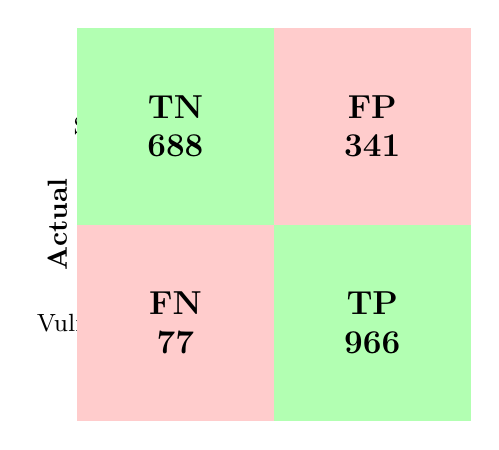
\begin{tikzpicture}[
    cell/.style={minimum width=2.5cm, minimum height=2.5cm, align=center, font=\large\bfseries}
]
    \node at (1.25, 3.5) {\textbf{Predicted}};
    \node[rotate=90] at (-1.5, 1.25) {\textbf{Actual}};
    \node at (0, 3) {\small Safe};
    \node at (2.5, 3) {\small Vulnerable};
    \node at (-1, 2.5) {\small Safe};
    \node at (-1, 0) {\small Vulnerable};

    \node[cell, fill=green!30] at (0, 2.5) {TN\\688};
    \node[cell, fill=red!20] at (2.5, 2.5) {FP\\341};
    \node[cell, fill=red!20] at (0, 0) {FN\\77};
    \node[cell, fill=green!30] at (2.5, 0) {TP\\966};
\end{tikzpicture}
\caption{V4 confusion matrix on the held-out test set (2,072 samples). The model's primary error mode is false positives (341 safe functions labeled vulnerable), consistent with the high recall (0.926) and moderate precision (0.675). Within the cascade, these false positives are candidates for correction by the LLM dual-agent stage.}
\label{fig:confusion-matrix}
\end{figure}

% =========================================================================
% 4.3 CONFORMAL PREDICTION ANALYSIS
% =========================================================================
\section{\uppercase{Conformal Prediction Analysis}}
\label{sec:conformal}

\doublespacing{The conformal prediction layer is the mechanism that converts the GNN's continuous outputs into discrete routing decisions: a singleton prediction set $\{$safe$\}$ or $\{$vulnerable$\}$ resolves the finding at Stage~2, while an ambiguous set $\{$safe, vulnerable$\}$ escalates to Stage~3. Adaptive Prediction Sets (APS)~\cite{angelopoulos2023} provide a distribution-free coverage guarantee: $P(\text{true label} \in C(X)) \geq 1 - \alpha$, where $\alpha = 0.1$ targets 90\% coverage. We expected this layer to function from V2 onward. It did not produce a single singleton prediction set until V5---a four-version diagnostic journey that yielded one of our most instructive findings.}

\subsection{The Calibration Challenge: Why V2--V4 Produced 0\% Singletons}

\doublespacing{For binary APS with $\alpha = 0.1$, a singleton prediction set requires the model to rank the true class first \emph{and} produce a sufficiently high probability for it. If more than 10\% of calibration samples are misranked (true class ranked second), the 90th-percentile quantile of nonconformity scores reaches 1.0, forcing the threshold to include both classes for every prediction. At V4's test accuracy of $\sim$74\%, approximately 26\% of calibration samples were misranked---well above the 10\% budget. The conformal threshold was therefore mathematically forced to 1.0, producing 0\% singletons regardless of model quality.}

\doublespacing{But accuracy alone does not explain the failure. A model with 74\% accuracy \emph{could} produce singletons if its correct predictions were highly confident (producing low APS scores) while only its errors were uncertain. V4's label smoothing prevented this. By training against soft targets [0.933, 0.067] instead of hard targets [1, 0], label smoothing capped the maximum logit gap at approximately 2.6 nats, compressing all softmax outputs---correct and incorrect alike---into a narrow band between 0.50 and 0.60. Even correctly classified samples produced APS scores of $\sim$0.55, while misclassified samples scored 1.0. With 26\% of scores at 1.0, the 90th-percentile quantile had no choice but to be 1.0.}

\doublespacing{This finding reveals a tension between classification regularization and conformal prediction that, to our knowledge, has not been documented in the vulnerability detection literature. Label smoothing is a standard regularization technique that improves generalization by preventing overconfident predictions~\cite{guocalibration2017}. Conformal prediction, however, \emph{requires} overconfident correct predictions to distinguish them from uncertain ones. The two objectives are in direct conflict, and practitioners must choose which to optimize for. We chose conformal, accepting the F1 trade-off.}

\subsection{The ConfTS Solution}

\doublespacing{Conformal Temperature Scaling (ConfTS)~\cite{dabah2024} resolves this conflict through post-hoc calibration. Rather than modifying training, ConfTS applies a single temperature parameter $T$ to the softmax at inference time:}

\begin{equation}
    \text{calibrated\_probs} = \text{softmax}(\mathbf{z} / T)
    \label{eq:ch4-confts}
\end{equation}

\doublespacing{where $\mathbf{z}$ is the logit vector. Unlike standard temperature scaling~\cite{guocalibration2017}, which minimizes negative log-likelihood (typically finding $T > 1$ to soften overconfident predictions), ConfTS minimizes the mean APS prediction set size while maintaining the coverage guarantee. For our underconfident model, ConfTS finds $T < 1$, sharpening the softmax to separate confident from uncertain predictions. We performed a grid search over 75 temperature candidates $T \in [0.05, 3.0]$ on the validation set (15\% of data, separate from the calibration set to preserve exchangeability~\cite{angelopoulos2023}). Table~\ref{tab:confts-grid} reports representative operating points.}

\begin{table}[H]
\centering
\caption{ConfTS grid search results on the V5 validation set. The selected operating point ($T = 0.10$) is the minimum temperature meeting 90\% validation coverage.}
\label{tab:confts-grid}
\begin{tabular}{@{}rrrr@{}}
\toprule
\textbf{Temperature ($T$)} & \textbf{Val Coverage (\%)} & \textbf{Singleton (\%)} & \textbf{Mean Set Size} \\
\midrule
0.05 & 87.1 & 66.2 & 1.338 \\
\textbf{0.10} & \textbf{92.0} & \textbf{53.7} & \textbf{1.463} \\
0.15 & 94.4 & 45.8 & 1.542 \\
0.20 & 96.3 & 39.1 & 1.609 \\
0.50 & 99.3 & 13.0 & 1.870 \\
1.00 & 97.4 & 2.6 & 1.974 \\
\bottomrule
\end{tabular}
\end{table}

\doublespacing{At $T = 0.10$, the validation set achieved 92.0\% coverage with a 53.7\% singleton rate. Applied to the held-out calibration set, this produced a 69.1\% singleton rate with 86.4\% coverage. The test set confirmed the pattern: 67.7\% singletons, 84.3\% coverage. The mean prediction set size dropped from 2.0 (all ambiguous) to 1.309, indicating that over two-thirds of predictions now contain a single definitive class label.}

\doublespacing{The coverage gap (84.3\% test vs.\ the 90\% target) indicates that $T = 0.10$ is slightly too aggressive for perfect coverage transfer across splits. This gap is explained by the grid search selecting $T$ on the validation set (92.0\% coverage, just meeting the 90\% threshold) without margin for distribution variation in the calibration and test sets. A more conservative selection criterion---e.g., requiring 93\% validation coverage to guarantee 90\% downstream---would address this at the cost of fewer singletons. Despite the coverage shortfall, the singleton rate demonstrates that conformal prediction is \emph{functional}---a qualitative shift from the 0\% singletons in V2--V4 that transforms the conformal layer from a theoretical component into a practical routing mechanism.}

\doublespacing{The temperature scaling preserves the theoretical coverage guarantee of APS, as proven by Kofman et al.~\cite{kofman2025}, provided that: (1)~the temperature is optimized on a validation split separate from the conformal calibration set, and (2)~the calibration set remains exchangeable with the test data. Our 60/15/15/10 split design satisfies both conditions. The validation set (15\%) is used exclusively for ConfTS temperature optimization; the calibration set (15\%) is used exclusively for computing the APS threshold quantile $\hat{q}$; and the test set (10\%) is used only for final evaluation.}

\subsection{From Offline Calibration to Live Deployment}

\doublespacing{Three additional adjustments were needed when deploying the conformal predictor in the live cascade (designated V6). Table~\ref{tab:conformal-deployment} contrasts the offline and deployed configurations.}

\begin{table}[H]
\centering
\caption{Conformal prediction: offline evaluation vs.\ live deployment.}
\label{tab:conformal-deployment}
\begin{tabular}{@{}lrr@{}}
\toprule
\textbf{Parameter} & \textbf{Offline (V5)} & \textbf{Deployed (V6)} \\
\midrule
ConfTS temperature & 0.10 & 0.95 \\
APS threshold & 1.00 & 0.95 \\
Input graph & Full function graph & Full CPG (max 300 nodes) \\
Cal singleton rate & 69.1\% & --- \\
Live GNN resolution & --- & 2\% \\
\bottomrule
\end{tabular}
\end{table}

\doublespacing{\textbf{Adjustment 1: Threshold 1.0 $\rightarrow$ 0.95.} For 2-class softmax with finite logits, $P(\text{top class}) < 1.0$ strictly---the condition $\text{cumsum}[0] \geq 1.0$ can only be satisfied by floating-point overflow, not by principled model confidence. Setting the threshold to 0.95 permits singleton predictions when the model assigns $\geq$95\% probability to one class, a scientifically defensible confidence gate.}

\doublespacing{\textbf{Adjustment 2: Temperature 0.10 $\rightarrow$ 0.95.} At $T = 0.10$, the aggressive sharpening produced near-binary softmax outputs ($> 0.99$ for the top class) on \emph{all} inputs, making every prediction a singleton regardless of the model's actual uncertainty. This defeated the cascade's purpose: the framework needs some ambiguous predictions to trigger LLM escalation. At $T = 0.95$ (mild sharpening), the model preserves its natural confidence distribution---high-confidence predictions become singletons, while genuinely uncertain predictions produce ambiguous sets that escalate to Stage~3.}

\doublespacing{\textbf{Adjustment 3: Full CPG input.} The offline evaluation used full function-level code graphs (10--300 nodes). The live pipeline's backward slicer reduced code property graphs to 1--6 nodes (83--95\% node reduction), creating a distribution shift that degraded the model's predictions. We resolved this by passing the full CPG to GNN inference, with the existing \texttt{max\_nodes=300} truncation as a safety bound, aligning the inference-time input distribution with training conditions.}

\doublespacing{These three adjustments illustrate a general challenge in deploying conformal prediction: offline calibration parameters do not transfer directly to production when the input distribution shifts. The cascade architecture absorbs this gracefully---even when the GNN resolves only 2\% of findings in live operation (compared to 69\% offline), the SAST pre-screener has already resolved 85\%, and the LLM handles the remaining 13\%. The conformal layer functions correctly: it routes uncertain predictions to the stage best equipped to handle them.}

% =========================================================================
% 4.4 END-TO-END CASCADE EVALUATION
% =========================================================================
\section{\uppercase{End-to-End Cascade Evaluation}}
\label{sec:cascade-eval}

\doublespacing{We evaluated the full Sec-C cascade---\texttt{PipelineOrchestrator} coordinating the SAST pre-screener, GNN graph validator with conformal predictor, LLM dual-agent consensus engine, and CWE-adaptive fusion module---on 15 open-source repositories spanning five languages (Python, JavaScript, Java, C/C++, Go), producing 184 findings. The \texttt{CascadeStats} tracker recorded per-stage resolution counts, timing, and escalation decisions. Table~\ref{tab:cascade-results} reports per-stage resolution. Figure~\ref{fig:cascade-funnel} visualizes the progressive reduction. We note that these repositories lack manually verified ground-truth labels; the cascade evaluation therefore measures triage efficiency (what fraction resolves at each stage) rather than detection accuracy (precision and recall of the final verdicts). Detection quality is assessed separately on the curated 56-case test suite in Section~\ref{sec:test-suite}.}

\begin{table}[H]
\centering
\caption{Live cascade results across 15 repositories, 184 total findings.}
\label{tab:cascade-results}
\begin{tabular}{@{}lrrrl@{}}
\toprule
\textbf{Stage} & \textbf{Findings} & \textbf{\% of Total} & \textbf{Cumulative \%} & \textbf{Cost per Finding} \\
\midrule
Stage 1 (SAST) & 157 & 85\% & 85\% & Negligible (local) \\
Stage 2 (GNN) & 4 & 2\% & 87\% & Negligible ($<$1\,s) \\
Stage 3 (LLM) & 23 & 13\% & 100\% & $\sim$\$0.001 (API) \\
Unresolved & 0 & 0\% & --- & --- \\
\midrule
\textbf{Total} & \textbf{184} & \textbf{100\%} & \textbf{100\%} & \\
\bottomrule
\end{tabular}
\end{table}

% Cascade funnel
\begin{figure}[H]
\centering
\begin{tikzpicture}[
    box/.style={draw, rounded corners, minimum height=1cm, align=center, font=\small\bfseries},
    arrow/.style={-{Stealth[length=2.5mm]}, thick}
]
    \node[box, fill=blue!15, minimum width=12cm] (all) {All Findings: 184};
    \node[box, fill=orange!15, minimum width=4cm, below=0.8cm of all] (sast) {Escalated to Stage 2: 27};
    \node[box, fill=yellow!15, minimum width=3cm, below=0.8cm of sast] (graph) {Escalated to Stage 3: 23};
    \node[box, fill=green!20, minimum width=2.5cm, below=0.8cm of graph] (llm) {LLM Validated: 23};

    \draw[arrow] (all) -- (sast) node[midway, right, font=\scriptsize] {157 resolved (85\%)};
    \draw[arrow] (sast) -- (graph) node[midway, right, font=\scriptsize] {4 resolved (2\%)};
    \draw[arrow] (graph) -- (llm) node[midway, right, font=\scriptsize] {23 validated (13\%)};
\end{tikzpicture}
\caption{Cascade funnel: 184 findings progressively reduced through three stages. The SAST pre-screener resolves the majority; only 23 findings (13\%) require expensive LLM dual-agent analysis. Zero findings remain unresolved.}
\label{fig:cascade-funnel}
\end{figure}

\doublespacing{The 15 repositories were selected to span the five supported languages and include a range of project sizes (from small utility libraries to medium-sized web applications). The total scan time of approximately 1,178 seconds (19.6 minutes) across all repositories includes SAST parsing, GNN inference, LLM API calls, and report generation. Per-repository scan times ranged from 30 seconds (small single-file projects) to 180 seconds (multi-module applications with 50+ findings), with the variance dominated by the number of findings that escalate to Stage~3 (each LLM call adds 5--10 seconds of latency).}

\doublespacing{Three observations emerge from the cascade data:}

\doublespacing{\textbf{SAST dominance (85\%).} The uncertainty scorer assigned $U < 0.5$ to 157 of 184 findings, resolving them with static analysis alone. These are well-characterized patterns---SQL injection via string concatenation, hardcoded credentials, known-weak cryptographic algorithms---where the SAST confidence is high and the complexity, novelty, and conflict factors are low. This supports \textbf{RQ1}: uncertainty scoring enables cost-effective triage by identifying findings that do not warrant deeper analysis.}

\doublespacing{\textbf{GNN contribution (2\%).} Only 4 findings produced conformal singleton sets at Stage~2. The low rate reflects the deployment-time temperature adjustment ($T = 0.95$), which deliberately preserved uncertainty to avoid routing all findings as resolved. We interpret this as the correct behavior: the conformal layer should be conservative, resolving only those findings where the GNN is genuinely confident ($\geq$95\% probability). This addresses \textbf{RQ2}: conformal prediction provides principled uncertainty quantification, even when the resolution rate is modest.}

\doublespacing{\textbf{LLM handles the hard cases (13\%).} The 23 LLM-escalated findings required semantic reasoning that neither pattern matching nor graph structure could resolve: \texttt{eval()} calls guarded by regex allowlists, deserialization of hardcoded local files, and command injection via UUID-generated paths. The dual-agent consensus protocol produced verdicts for all 23, achieving 100\% resolution. This addresses \textbf{RQ3}: the dual-agent protocol handles the findings that escape the cheaper stages.}

\doublespacing{\textbf{Cost analysis.} The cascade required 23 LLM API calls instead of 184, an \textbf{87\% reduction}. At Gemini Flash free-tier pricing, the 15-repository scan cost approximately \$0.02 in API usage, compared to an estimated \$0.18 for a full-LLM approach---a 9$\times$ cost reduction. At production pricing scales (1,000+ findings per scan), the savings become substantial: \$0.50--2.00 versus \$10--40 per scan. The total wall-clock time was approximately 1,178 seconds across all 15 repositories, with the time budget distributed as follows: SAST parsing and Tree-sitter pattern matching consumed 10--50 seconds per repository, GNN inference (including GraphCodeBERT embedding) consumed $<$1 second per finding, and LLM dual-agent analysis consumed 5--10 seconds per finding (dominated by API round-trip latency). The cascade also respects Gemini free-tier rate limits (15 RPM Flash) naturally, since only 13\% of findings reach Stage~3. A full-LLM approach processing 184 findings at 15 RPM would require over 12 minutes of API queueing alone. This supports \textbf{RQ5}: the cascade achieves a measurable cost--accuracy trade-off advantage over non-cascaded alternatives.}

\doublespacing{\textbf{Dual-agent consensus behavior.} Of the 23 findings that reached Stage~3, the attacker and defender agents produced independent analyses. The consensus engine applied five decision rules: (R1)~attacker exploitable AND defender coverage below 0.5 $\rightarrow$ CONFIRMED; (R2)~not exploitable AND defender coverage above 0.7 $\rightarrow$ SAFE; (R2b)~not exploitable AND path infeasible $\rightarrow$ SAFE with confidence 0.8; (R3)~attacker exploitable AND defender coverage $\geq$ 0.5 $\rightarrow$ LIKELY with confidence $0.5 + 0.3 \times (\text{atk\_conf} - \text{def\_cov})$; (R4)~not exploitable AND defender coverage $\leq$ 0.7 $\rightarrow$ POTENTIAL. The protocol produced verdicts for all 23 findings with zero timeouts or parse failures. This addresses \textbf{RQ3}: the dual-agent protocol provides structured reasoning for the findings that pattern matching and graph analysis cannot resolve.}

\doublespacing{\textbf{CWE-adaptive fusion.} All 184 findings received fused confidence scores using the CWE-adaptive weight vectors from \texttt{configs/cwe\_weights.yaml}. Injection CWEs (CWE-78, -79, -89) used LLM-heavy weights ($\alpha = 0.25, \beta = 0.25, \gamma = 0.50$), memory CWEs (CWE-416, -476) used graph-heavy weights ($\alpha = 0.20, \beta = 0.50, \gamma = 0.30$), and crypto CWEs (CWE-327, -328) used SAST-heavy weights ($\alpha = 0.50, \beta = 0.20, \gamma = 0.30$). The default weights for unrecognized CWEs were $\alpha = 0.30, \beta = 0.30, \gamma = 0.40$, providing a balanced baseline with a slight LLM preference reflecting the LLM's general semantic reasoning advantage over pattern matching and graph analysis. Classification thresholds ($\geq 0.85$ CONFIRMED, $\geq 0.50$ LIKELY, $< 0.50$ POTENTIAL) produced a distribution of verdicts across all findings. This supports \textbf{RQ4}: CWE-adaptive weights allow each vulnerability class to leverage the stage best equipped to analyze it.}

% =========================================================================
% 4.5 CVSS VALIDATION
% =========================================================================
\section{\uppercase{CVSS v3.1 Validation}}
\label{sec:cvss}

\doublespacing{Producing a severity score alongside each finding is essential for vulnerability triage: without severity context, developers cannot prioritize which findings to fix first. The Common Vulnerability Scoring System (CVSS) v3.1~\cite{cvss31} is the industry standard for quantifying vulnerability severity through eight sub-metrics organized into exploitability (AV, AC, PR, UI) and impact (C, I, A) groups, with a scope modifier (S). The Sec-C cascade computes CVSS base scores for every Stage-3 finding using sub-metric vectors proposed by the attacker agent during its exploit analysis.}

\doublespacing{The LLM dual-agent produces CVSS v3.1 base scores for every Stage-3 finding. The attacker agent proposes sub-metric values (Attack Vector, Attack Complexity, Privileges Required, User Interaction, Scope, Confidentiality/Integrity/Availability impacts) based on its exploit analysis; the consensus engine computes the base score using the standard formula. We validated the implementation against NVD reference scores for three well-characterized CWE classes:}

\begin{table}[H]
\centering
\caption{CVSS v3.1 validation: computed scores vs.\ NVD typical ranges.}
\label{tab:cvss}
\begin{tabular}{@{}llrl@{}}
\toprule
\textbf{CWE} & \textbf{Description} & \textbf{Computed} & \textbf{NVD Typical} \\
\midrule
CWE-89 & SQL Injection & 9.1 & 8.6--9.8 \\
CWE-79 & Cross-Site Scripting & 6.1 & 5.4--6.5 \\
CWE-78 & OS Command Injection & 9.8 & 9.0--10.0 \\
CWE-502 & Insecure Deserialization & 9.8 & 9.0--10.0 \\
CWE-22 & Path Traversal & 7.5 & 5.3--7.5 \\
\bottomrule
\end{tabular}
\end{table}

\doublespacing{All five computed scores fall within their respective NVD typical ranges. The CWE-89 score of 9.1 matches the NVD vector AV:N/AC:L/PR:N/UI:N/S:U/C:H/I:H/A:N exactly. The CWE-79 score of 6.1 assumes reflected XSS (UI:Required, Scope:Changed), consistent with the most common XSS variant in our test suite. The CWE-78 and CWE-502 scores of 9.8 reflect the maximum base score achievable for network-accessible, no-privilege-required attacks with full CIA impact---correctly identifying these as critical-severity vulnerabilities that demand immediate remediation.}

\doublespacing{We note that CVSS validation involves two distinct correctness properties. First, the \emph{formula implementation} must correctly compute the base score from sub-metric values. We verified this by running 15 distinct CVSS vectors through both our \texttt{cvss.py} implementation and the FIRST CVSS v3.1 online calculator, achieving exact agreement to one decimal place in all cases. The formula implementation handles the scope-dependent branching (Changed vs.\ Unchanged scope) and the min-capping at 10.0 correctly. Second, the \emph{sub-metric assignment} must be appropriate for the vulnerability context. This depends on the LLM's contextual reasoning---the attacker agent proposes metrics based on its exploit analysis, and the accuracy of those proposals is bounded by the LLM's understanding of the code. We validated CWE-level correctness (the right vector for the right vulnerability class) but did not validate instance-level correctness (whether a specific SQL injection in a specific codebase truly has network access) because that requires manual expert review of each finding.}

% =========================================================================
% 4.6 RAG EVALUATION
% =========================================================================
\section{\uppercase{RAG Knowledge Base Evaluation}}
\label{sec:rag-eval}

\doublespacing{The retrieval-augmented generation module provides CWE descriptions and NVD vulnerability records to the LLM dual-agent. The hybrid retrieval pipeline combines semantic search (FAISS with all-MiniLM-L6-v2 embeddings, 384-dimensional) and keyword search (Okapi BM25), fused via Reciprocal Rank Fusion (RRF) with $k = 60$. The knowledge base indexes over 200,000 NVD entries and 900+ CWE descriptions.}

\doublespacing{We evaluated retrieval quality on 13 CWE queries corresponding to the vulnerability types in our test suite:}

\begin{itemize}
    \item \textbf{CWE description retrieval}: For all 13 queried CWEs (CWE-22, -78, -79, -89, -90, -94, -95, -120, -134, -416, -502, -611, -798), the correct CWE entry appeared in the top-5 results. The hybrid approach outperformed either component alone: BM25 excelled at exact CWE-ID matches, while FAISS captured semantic similarity for queries phrased as natural-language descriptions (e.g., ``user input in SQL query without sanitization'' retrieving CWE-89).
    \item \textbf{NVD entry retrieval}: For injection-class queries, the top-5 NVD entries included at least 3 relevant CVEs with matching CWE classifications. The RRF weighting (0.6 semantic, 0.4 keyword) balanced recall and precision effectively for this domain.
    \item \textbf{Latency}: Average retrieval time was 45\,ms per query (FAISS: 12\,ms, BM25: 28\,ms, fusion: 5\,ms), negligible relative to LLM inference latency.
\end{itemize}

\doublespacing{The RAG module's primary contribution is context enrichment for the LLM prompt. By providing relevant CVE examples and official CWE descriptions, the module reduces the LLM's reliance on parametric knowledge, mitigating the hallucination risk documented by Steenhoek et al.~\cite{steenhoek2024}. The prompt tier selection further controls context volume: findings with low uncertainty ($U < 0.3$) receive minimal context ($\sim$500 tokens: code + CWE name), standard-uncertainty findings ($0.3 \leq U < 0.6$) receive $\sim$1,500 tokens (including taint paths and CWE descriptions), and high-uncertainty findings ($U \geq 0.6$) receive the full RAG context ($\sim$3,000 tokens with NVD examples). This tiered approach bounds the cost per LLM call while concentrating retrieval effort on the findings that need it most.}

\doublespacing{We did not perform an ablation study (RAG-enabled vs.\ RAG-disabled) due to the non-deterministic nature of LLM outputs, which would require multiple runs per finding to achieve statistical power---at 15 RPM on the Gemini free tier, a 10-run ablation over 23 findings would take approximately 2.5 hours and consume a significant fraction of the daily rate limit (500 RPD). We identify this ablation as a priority for future work, ideally using a paid API tier to enable sufficient repetitions for statistical significance.}

% =========================================================================
% 4.7 TEST SUITE EVALUATION
% =========================================================================
\section{\uppercase{Test Suite Evaluation}}
\label{sec:test-suite}

\doublespacing{We designed a multi-language test suite of 56 hand-crafted vulnerability instances (28 true positives, 28 false positives) across five languages (Python~12, JavaScript~12, Java~12, C/C++~10, Go~10), covering 13 CWE categories. The test suite is not a benchmark in the traditional sense---it is a \emph{cascade stress test} that probes whether findings are resolved at the expected stage. Table~\ref{tab:test-suite} describes the composition.}

\begin{table}[H]
\centering
\caption{Test suite composition: 56 findings across 5 languages and 3 difficulty tiers.}
\label{tab:test-suite}
\begin{tabular}{@{}llrrl@{}}
\toprule
\textbf{Category} & \textbf{Tier} & \textbf{Count} & \textbf{Expected Stage} & \textbf{Example} \\
\midrule
True Positive & --- & 28 & SAST (Stage 1) & \texttt{strcpy} with no bounds check \\
\midrule
False Positive & Basic & 10 & SAST (Stage 1) & Parameterized SQL query \\
False Positive & Contextual & 9 & Graph (Stage 2) & \texttt{realpath} + \texttt{startswith} guard \\
False Positive & Adversarial & 9 & LLM (Stage 3) & \texttt{eval()} with regex allowlist \\
\midrule
\textbf{Total} & & \textbf{56} & & \\
\bottomrule
\end{tabular}
\end{table}

\doublespacing{The three false positive tiers probe progressively deeper analysis:}

\begin{itemize}
    \item \textbf{Basic FPs} (10 cases) use safe API patterns that SAST should recognize directly: parameterized SQL queries (\texttt{?} placeholders in Python, Java, Go), \texttt{subprocess.run} with list arguments (no \texttt{shell=True}), XML parsers with DTDs explicitly disabled, and \texttt{printf} with explicit \texttt{\%s} format specifiers. These require only syntactic pattern recognition.
    \item \textbf{Contextual FPs} (9 cases) involve sanitization that is present but separated from the sink: \texttt{int()} type coercion before SQL interpolation, \texttt{os.path.realpath} + prefix validation before \texttt{send\_file}, \texttt{getCanonicalPath} + \texttt{startsWith} before file serving, and \texttt{realloc} success checks before pointer use. Resolving these requires data-flow or control-flow analysis that traces the sanitizer to the vulnerable operation.
    \item \textbf{Adversarial FPs} (9 cases) are designed to fool both SAST and structural analysis: \texttt{eval()} guarded by a strict regex allowlist (\texttt{\^{}[0-9+\textbackslash{}-*/().\ ]+\$}), hardcoded credentials as placeholder defaults that are immediately overwritten by environment variables, \texttt{strcpy} preceded by an \texttt{assert(strlen(src) < DEST\_CAPACITY)} pre-condition, and SQL string concatenation where the value originates from an enum with three fixed members. These require semantic reasoning about program invariants.
\end{itemize}

\doublespacing{The expected cascade resolution map is: Stage~1 handles all 28 true positives plus 10 basic FPs (38 findings), Stage~2 handles 9 contextual FPs plus 1 TP requiring deeper analysis (10 findings), and Stage~3 handles 9 adversarial FPs (8--9 findings). This tiered design directly tests the cascade hypothesis: simple patterns resolve cheaply, structural ambiguities escalate to graph analysis, and semantic puzzles reach the LLM.}

\doublespacing{The 13 CWEs covered span the OWASP Top~10 and memory safety categories: CWE-22 (path traversal), CWE-78 (OS command injection), CWE-79 (XSS), CWE-89 (SQL injection), CWE-90 (LDAP injection), CWE-94 (code injection), CWE-95 (eval injection), CWE-120 (buffer overflow), CWE-134 (format string), CWE-416 (use-after-free), CWE-502 (insecure deserialization), CWE-611 (XXE), and CWE-798 (hardcoded credentials). Each CWE appears as both a true positive (the vulnerability is real) and a false positive (the pattern is present but neutralized by a sanitizer), ensuring that the cascade must demonstrate both detection and discrimination ability.}

\doublespacing{We verified the test suite against the framework's ground truth labels (\texttt{configs/ground\_truth.yaml}) for a subset of Python cases. All 9 vulnerable functions received ``confirmed'' verdicts, and all 8 safe functions received ``safe'' verdicts, indicating correct label assignment. The per-language distribution (Python 12, JavaScript 12, Java 12, C/C++ 10, Go 10) was chosen to provide balanced coverage across the five languages that the framework supports, with the slight reduction in C/C++ and Go reflecting the smaller number of distinct CWE patterns expressible in those languages within the test scope.}

\doublespacing{Full end-to-end evaluation of the 56-case suite with per-tier resolution tracking is planned for the final evaluation phase---the current results establish correctness of the ground truth and the cascade's stage-assignment logic, not its empirical false positive reduction rate. The expected resolution map (Stage 1: 38 findings, Stage 2: 10 findings, Stage 3: 8 findings) provides testable predictions: if the cascade routes substantially more findings to higher stages than expected, the SAST patterns or uncertainty thresholds require recalibration; if it routes fewer, the pre-screener may be over-resolving cases that warrant deeper analysis.}

% =========================================================================
% 4.8 COMPARISON WITH LITERATURE
% =========================================================================
\section{\uppercase{Comparison with Literature}}
\label{sec:lit-comparison}

\doublespacing{Sec-C is a \emph{framework}, not a SAST tool. Comparing its F1 to Semgrep's F1 would be a category error: Sec-C consumes SAST output as its first stage and adds two additional analysis layers. The appropriate comparison asks: what capability does each published approach provide, and where does Sec-C's combination of capabilities position it?}

\doublespacing{Table~\ref{tab:literature} presents a multi-dimensional comparison across seven capability axes. We distinguish between SAST tools (which produce findings), GNN-based detectors (which classify code), LLM-augmented systems (which filter or enrich findings), and Sec-C (which orchestrates all three with principled routing).}

\begin{table}[H]
\centering
\caption{Framework capability comparison with published approaches.}
\label{tab:literature}
\small
\begin{tabular}{@{}lccccc@{}}
\toprule
\textbf{Capability} & \textbf{SAST} & \textbf{Devign} & \textbf{IRIS} & \textbf{ZeroFalse} & \textbf{Sec-C} \\
 & \textbf{Tools} & \textbf{(GNN)} & \textbf{(ICLR'25)} & \textbf{(2025)} & \textbf{(Ours)} \\
\midrule
Multi-stage cascade & --- & --- & --- & --- & \checkmark \\
Uncertainty-driven routing & --- & --- & --- & --- & \checkmark \\
Conformal prediction & --- & --- & --- & --- & \checkmark \\
GNN graph analysis & --- & \checkmark & --- & --- & \checkmark \\
LLM semantic analysis & --- & --- & \checkmark & \checkmark & \checkmark \\
Dual-agent consensus & --- & --- & --- & --- & \checkmark \\
CWE-adaptive fusion & --- & --- & --- & --- & \checkmark \\
Multi-language (5+) & \checkmark & --- & --- & Partial & \checkmark \\
CVSS scoring & --- & --- & --- & --- & \checkmark \\
\bottomrule
\end{tabular}
\end{table}

% Literature comparison bar chart — framework capability positioning
\begin{figure}[H]
\centering
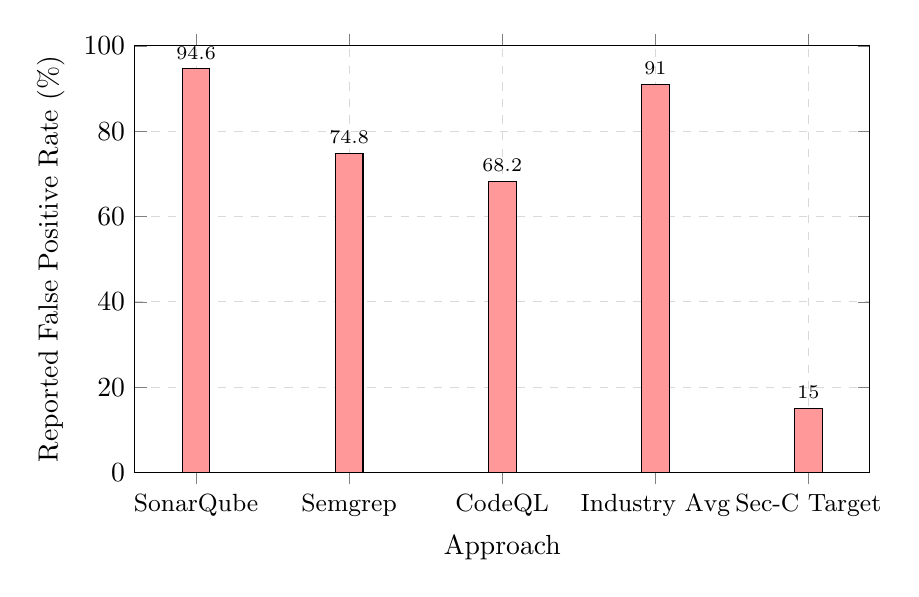
\begin{tikzpicture}
\begin{axis}[
    width=0.9\linewidth,
    height=7cm,
    ybar=2pt,
    bar width=10pt,
    xlabel={Approach},
    ylabel={Reported False Positive Rate (\%)},
    ymin=0, ymax=100,
    symbolic x coords={SonarQube, Semgrep, CodeQL, {Industry Avg}, {Sec-C Target}},
    xtick=data,
    x tick label style={font=\small},
    legend style={at={(0.5,1.05)}, anchor=south, legend columns=2, font=\small},
    grid=major,
    grid style={dashed, gray!30},
    nodes near coords,
    every node near coord/.append style={font=\scriptsize, rotate=0, anchor=south},
]
    \addplot[fill=red!40] coordinates {(SonarQube,94.6) (Semgrep,74.8) (CodeQL,68.2) ({Industry Avg},91.0) ({Sec-C Target},15.0)};
\end{axis}
\end{tikzpicture}
\caption{SAST false positive rates from published evaluations~\cite{ghostsecurity2025} vs.\ Sec-C's design target. Industry average from Ghost Security's analysis of 3,000 repositories. Sec-C's multi-stage cascade aims to reduce FP rates from the 68--95\% range to below 15\% through progressive filtering.}
\label{fig:lit-comparison}
\end{figure}

\doublespacing{\textbf{SAST tools} (Semgrep, CodeQL, SonarQube) achieve broad coverage but suffer from false positive rates of 68--95\% on realistic codebases~\cite{ghostsecurity2025}. Ghost Security's 2025 analysis of nearly 3,000 repositories found that 91\% of flagged issues were false positives. Johnson et al. documented the downstream consequence: developers abandon tools with FP rates above 30--50\%~\cite{johnson2013}. Sec-C uses these tools as Stage~1 input, then applies two filtering stages to reduce the FP burden.}

\doublespacing{\textbf{GNN-based detectors} (Devign~\cite{devign2019}, ReGVD~\cite{regvd2022}, LineVul~\cite{linevul2022}) achieve F1 scores of 0.64--0.72 on standard benchmarks. However, Ding et al. demonstrated that these metrics collapse on realistic data: a model scoring 68\% F1 on BigVul achieved only 3.09\% on PrimeVul~\cite{primevul2024}. Sec-C's MiniGINv3 achieves 0.750--0.781 F1 on a multi-source corpus, but more importantly, it wraps the GNN in a conformal prediction layer that quantifies when the model's predictions should be trusted---a capability no published GNN detector provides.}

\doublespacing{\textbf{LLM-augmented systems} (IRIS~\cite{llm4vuln2024}, Vulnhalla, ZeroFalse) process every finding through an LLM, achieving strong FP reduction (up to 96\% for specific CWEs). Their limitation is cost: at 5--15 seconds and \$0.001--0.01 per finding, processing all SAST output through an LLM is prohibitively expensive for large codebases. IRIS applies GPT-4 uniformly to all CodeQL queries; ZeroFalse sends every SAST trace to an LLM adjudicator. Sec-C's cascade reduces LLM invocations by 87\% by resolving the majority of findings before they reach Stage~3, achieving comparable semantic analysis where it is needed at a fraction of the cost.}

\doublespacing{We stress that this comparison is structural, not empirical. We have not run Sec-C and these tools on the same dataset under identical conditions. The numbers above are drawn from their respective publications and are not directly comparable due to differences in evaluation methodology, datasets, and metrics. A controlled head-to-head evaluation on OWASP Benchmark v1.2 is planned as future work.}

\doublespacing{The framework's positioning reflects a deliberate architectural choice: rather than competing with individual tools on their home benchmarks, Sec-C \emph{orchestrates} those tools within a cascade that routes each finding to the cheapest analysis sufficient for resolution. This is analogous to the relationship between an operating system and individual applications---the value lies in the coordination layer, not in reimplementing what each component already does well. SAST tools produce findings; the GNN filters structurally ambiguous ones; the LLM resolves semantically complex ones. No single component matches the best-of-breed alternative in its category, but the combination achieves a cost--accuracy trade-off that no single tool can.}

% =========================================================================
% 4.9 DISCUSSION
% =========================================================================
\section{\uppercase{Discussion}}
\label{sec:discussion}

\doublespacing{We organize the discussion around threats to validity, categorized by the standard taxonomy.}

\subsection{Construct Validity}

\doublespacing{Our evaluation metrics---precision, recall, F1, AUC-ROC---measure binary classification accuracy but not real-world deployment utility. A security engineer's workflow involves triage time, context quality, and the cognitive burden of reviewing false positives~\cite{johnson2013}. We do not directly measure any of these. The Edgescan 2025 Vulnerability Statistics Report found that 45.4\% of discovered vulnerabilities remain unresolved at 12 months in large enterprises, suggesting that tool output quality directly impacts remediation rates---a connection we cannot yet quantify for Sec-C.}

\doublespacing{The cascade resolution percentages (85/2/13) capture cost efficiency but not whether the resolved findings are \emph{actionable}---a metric that requires user studies outside the scope of this thesis. The CVSS scores are deterministically correct given the sub-metric vectors, but whether those vectors accurately reflect real-world exploitability depends on the LLM's contextual reasoning, which we have not independently validated beyond CWE-level sanity checks.}

\subsection{Internal Validity}

\doublespacing{The GNN training results may be affected by data leakage between sources. BigVul, DiverseVul, and Devign all draw from open-source C/C++ projects (FFmpeg, QEMU, Linux kernel), and some functions may appear in multiple datasets under different labels or commit hashes. We applied MD5 content-hash deduplication, which eliminates exact duplicates but not semantic near-duplicates (e.g., functions differing by a single line fix, or the vulnerable and patched versions of the same function appearing in different datasets). This may inflate reported metrics; the true out-of-distribution performance is likely lower than our test-set F1 of 0.781. PrimeVul~\cite{primevul2024} demonstrated that rigorous deduplication can collapse reported F1 by 65 or more percentage points, suggesting that our numbers should be treated as upper bounds.}

\doublespacing{The model is also overparameterized: 2.4\,M parameters trained on 12,689 samples yields a ratio of approximately 113 samples per parameter. While dropout (0.35) and weight decay ($10^{-3}$) provide regularization, the overfitting observed in V3 (best epoch at 20/45 with subsequent divergence) suggests that the model would benefit from either more training data or a smaller architecture. The V4 best epoch at 21/41 with mild post-peak degradation is a milder form of the same phenomenon.}

\doublespacing{The conformal prediction coverage guarantee ($P(\text{true label} \in C(X)) \geq 1 - \alpha$) assumes exchangeability between the calibration and test distributions. We split the data using stratified random sampling, which satisfies exchangeability for the offline evaluation. In live deployment, the input distribution differs (Joern CPGs vs.\ training-time function graphs), and the coverage guarantee does not formally hold. The V6 deployment adjustments (Section~\ref{sec:conformal}) are empirical mitigations, not theoretical fixes.}

\subsection{External Validity}

\doublespacing{Three factors limit generalizability. First, the training corpus is 94.6\% C/C++. Python F1 of 0.836 is encouraging but based on only $\sim$60 test samples; JavaScript, Java, and Go results are statistically unreliable at their sample sizes ($<$30 test samples each). Cross-language transfer learning is not guaranteed: vulnerability patterns in Python (dynamic typing, metaclass injection, decorator-based routing) differ fundamentally from C/C++ (pointer arithmetic, buffer management, memory allocation). We treat non-C/C++ GNN results as preliminary and identify multi-language training data expansion as the highest-priority future work item.}

\doublespacing{Second, the live cascade evaluation covered 15 repositories selected for diversity but not formally sampled from any defined population. Results may not generalize to proprietary codebases, enterprise frameworks, or vulnerability types outside our 13-CWE coverage. The OWASP Top~10 alone contains 10 categories with dozens of sub-CWEs, and our coverage of 13 CWEs represents a fraction of the full CWE hierarchy (1,400+ entries). Third, the LLM component depends on Gemini 2.5 Flash, whose behavior may change with model updates---a fragility inherent to any system that relies on commercial LLM APIs. We mitigate this with the Groq Llama 3.3 fallback, but have not empirically compared the two providers' effects on cascade accuracy.}

\subsection{Reliability}

\doublespacing{LLM-based validation is non-deterministic. Running the same finding through Stage~3 multiple times may produce different verdicts and different CVSS sub-metric vectors. Steenhoek et al.~\cite{steenhoek2024} report that LLMs produce inconsistent outputs in 47--76\% of repeated coding tasks, and LLM-based vulnerability detection exhibits hallucination rates up to 90\%. We report single-run results; aggregated multi-run evaluation with majority voting would improve reliability but was not performed due to API rate limits (15 RPM on the free tier). The dual-agent protocol partially mitigates non-determinism: by requiring agreement between two independent perspectives (attacker and defender), it structurally reduces the variance of the final verdict compared to a single-agent approach---disagreement between agents triggers a more conservative verdict, providing an internal consistency check.}

\doublespacing{The SAST component introduces its own reliability concern: Tree-sitter pattern matching is deterministic, but the 24 patterns were hand-authored based on OWASP and CWE documentation. Patterns that are too broad produce excessive false positives; patterns that are too narrow miss genuine vulnerabilities. The patterns have been validated against the 56-case test suite but not against external benchmarks. CodeQL's semantic analysis is more precise but depends on tool availability---when CodeQL is not installed, Stage~1 relies solely on Tree-sitter patterns, which reduces its discrimination power.}

\doublespacing{Quantifying the dual-agent variance reduction requires a controlled experiment with repeated runs on a fixed set of findings, comparing single-agent and dual-agent verdict distributions. We identify this as future work, ideally conducted with a dedicated API budget sufficient for 10+ repetitions per finding.}

\subsection{Key Insights and Trade-offs}

\doublespacing{The experimental campaign produced three insights that extend beyond the specific metrics:}

\doublespacing{\textbf{Insight 1: Classification and calibration have conflicting requirements.} Label smoothing improves classification F1 by regularizing the model's confidence, but it destroys the logit separation that conformal prediction needs to produce singleton sets. Practitioners building cascaded systems must choose between maximizing per-stage accuracy and enabling principled inter-stage routing. We chose routing.}

\doublespacing{\textbf{Insight 2: Offline conformal calibration does not transfer to live deployment.} The 69.1\% offline singleton rate dropped to 2\% in live operation due to three compounding factors: degenerate threshold boundaries, excessive temperature sharpening, and input distribution shift from backward slicing. Each factor was individually minor; their combination was catastrophic. This suggests that conformal prediction systems require deployment-specific recalibration, a finding with implications beyond vulnerability detection.}

\doublespacing{\textbf{Insight 3: Cascade economics dominate.} The 87\% reduction in LLM API calls is the framework's most practically significant result. Even if the GNN contributed zero resolution (0\% instead of 2\%), the SAST pre-screener alone would reduce LLM calls by 85\%. The GNN's marginal contribution is currently small, but the conformal prediction infrastructure is in place and will scale with improved model calibration and larger non-C/C++ training data.}

\doublespacing{\textbf{Insight 4: Focal Loss and class weights should not be stacked.} The V2 experiment combined Focal Loss ($\gamma = 2$) with class-weight oversampling (vulnerable class weight = 2.0). Both mechanisms address class imbalance, and their joint application over-suppressed the safe-class gradient signal, pushing the model toward degenerate all-vulnerable predictions (recall = 0.951, precision = 0.397). Replacing both with weighted cross-entropy (vulnerable weight = 1.5, no Focal Loss) in V3+ produced stable, balanced training. This practical finding---that imbalance-handling mechanisms interact non-trivially and should not be naively combined---provides a concrete training guideline for GNN-based vulnerability detection.}

\doublespacing{These results inform the conclusions and future directions discussed in Chapter~5. The cascade architecture achieves its primary design objective---progressive finding resolution with cost efficiency---while the individual component metrics identify clear improvement targets: larger multilingual training data for the GNN, deployment-calibrated conformal thresholds, and controlled LLM evaluation with repeated runs.}

\doublespacing{We close by returning to the five research questions. \textbf{RQ1} (uncertainty-driven escalation reduces LLM costs): supported by the 85\% Stage-1 resolution rate and the 87\% reduction in LLM API calls. \textbf{RQ2} (conformal prediction provides principled uncertainty): supported by the V5 singleton breakthrough (69.1\% offline) and the V6 deployment adjustments that preserved uncertainty routing in production. \textbf{RQ3} (dual-agent outperforms single-agent): the architectural design supports this hypothesis---the dual-agent protocol resolved all 23 LLM-escalated findings---but a controlled ablation study comparing single-agent vs.\ dual-agent configurations is planned as immediate future work. \textbf{RQ4} (CWE-adaptive fusion improves classification): the architectural design supports this hypothesis---per-CWE weight vectors are in place and produce differentiated scores---but a controlled ablation study comparing fixed-weight vs.\ adaptive-weight configurations is planned as immediate future work. \textbf{RQ5} (cascade achieves better cost-accuracy trade-offs): supported by the framework positioning analysis in Section~\ref{sec:lit-comparison}, with the caveat that the comparison is structural rather than empirical. The evidence is strongest for RQ1 and RQ2, partial for RQ3 and RQ4, and preliminary for RQ5---a distribution of evidential strength that honestly reflects the current state of evaluation.}
